\documentclass[11pt,letterpaper]{article}
\usepackage[utf8]{inputenc}

%----- Configuración del estilo del documento------%
\usepackage{epsfig,graphicx}
\usepackage[left=2cm,right=2cm,top=1.8cm,bottom=2.3cm]{geometry}
\usepackage{fancyhdr}
\usepackage{lastpage}
\usepackage{url}
\pagestyle{fancy}
\fancyhf{}
\rfoot{\textit{Página \thepage \hspace{1pt} de \pageref{LastPage}}}


%------ Paquetes matemáticos básicos --------%
\usepackage{amsmath}
\usepackage{amssymb}
\usepackage{amsthm}

\usepackage[spanish]{babel}
\usepackage{graphicx}
\usepackage{hyperref}

\usepackage{tabularx}
\usepackage{xcolor}
\usepackage[table]{xcolor}
\usepackage{colortbl}
\usepackage{array, multirow, multicol, tabularx}
\usepackage{tcolorbox}
\newtheorem{theorem}{Theorem}[section]
\newtheorem{corollary}{Corollary}[theorem]
\newtheorem{lemma}[theorem]{Lemma}

%------si-------%
\definecolor{B}{HTML}{FFFFFF}
\definecolor{G}{HTML}{5e5e5e}
\definecolor{R2}{HTML}{d53d40}
\definecolor{A2}{HTML}{034190}
\definecolor{V2}{HTML}{7faa50}
\newcommand{\R}{\mathbb{R}}
\newcommand{\C}{\mathcal{C}}
\newcommand{\N}{\mathbb{N}}
\newcommand{\Z}{\mathbb{Z}}
\newcommand{\Q}{\mathbb{Q}}
\renewcommand{\theenumi}{\Roman{enumi}}
\renewcommand{\labelenumi}{{\theenumi}.}

\begin{document}

%------ Encabezado -------- %

\begin{center}
    \begin{minipage}{3cm}
    	\begin{center}
    		\includegraphics[height=3.4cm]{logo_unam.png}
    	\end{center}
    \end{minipage}\hfill
    \begin{minipage}{10cm}
    	\begin{center}
    	\textbf{\large Universidad Nacional Autónoma de México}\\[0.1cm]
        \textbf{Facultad de Ciencias}\\[0.1cm]
        \textbf{C\'alculo II}\\[0.1cm]
        Decimas extra\\[0.1cm]
         El\'ias L\'opez Rivera\\[0.1cm]
        \texttt{ elias.lopezr\,@ciencias.unam.mx }\\[0.1cm]
        Fecha:\,\,17/05/2025
    	\end{center}
    \end{minipage}\hfill
    \begin{minipage}{3cm}
    	\begin{center}
    		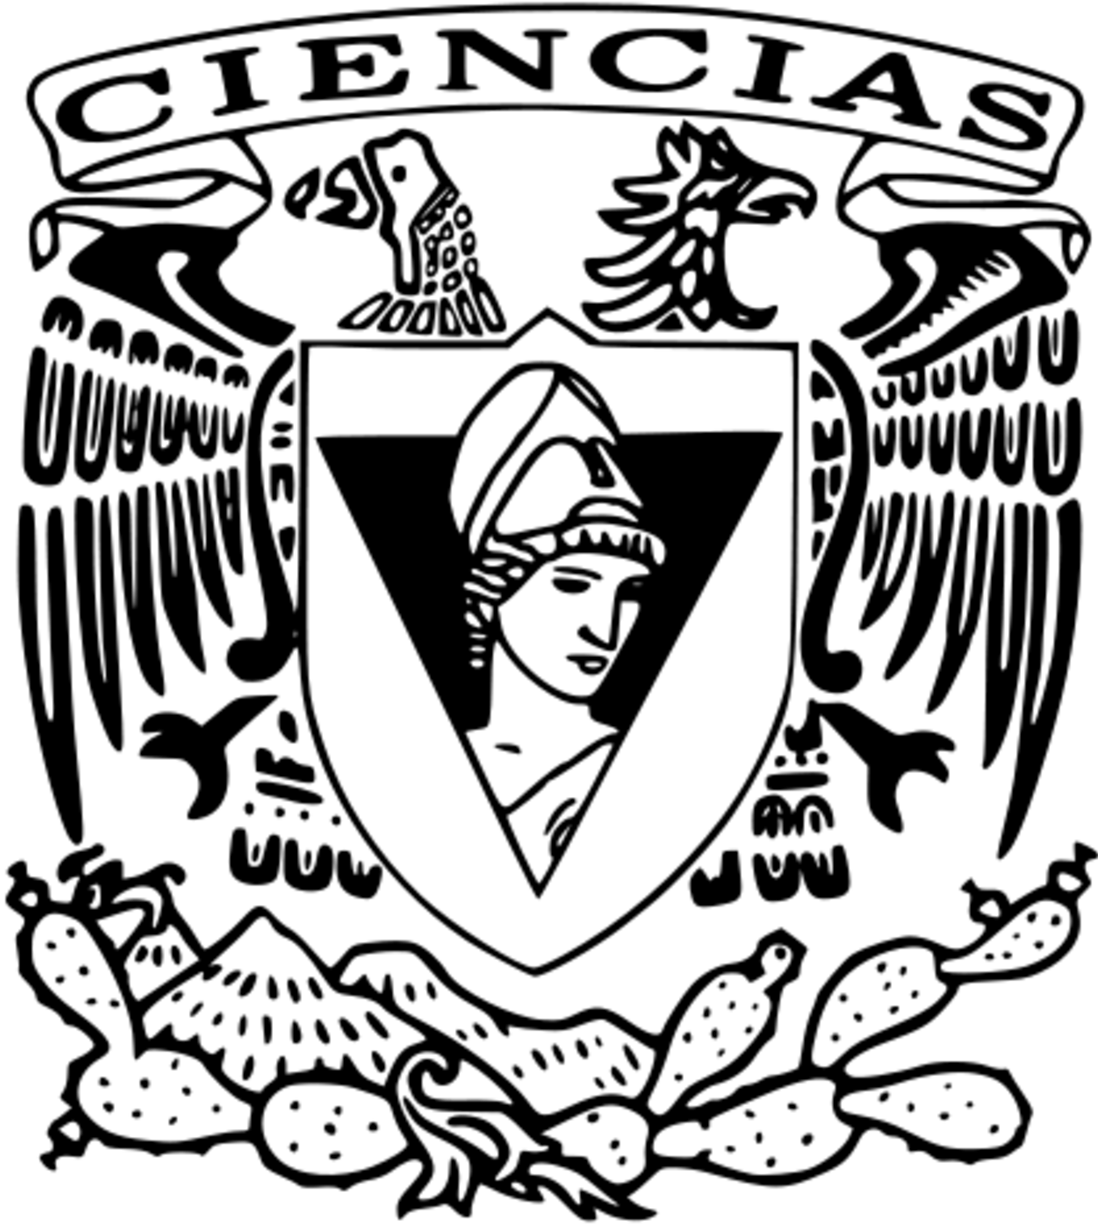
\includegraphics[height=3.4cm]{Logo_FC.png}
    	\end{center}
    \end{minipage}
\end{center}

\rule{17cm}{0.1mm}

%------ Fin de encabezado -------- %
\,\\
\begin{tcolorbox}[
	title = \textcolor{black}{\textcolor{white}{Problema}},]
\textit{Sea $\{a_n\}\subset \mathbb{R}$ una sucesi\'on tal que $a_n>0$ para toda $n\in \N$. Suponga que\,\\
\begin{equation*}
\displaystyle\,\lim_{n\rightarrow \infty}\,\frac{\log\left(\frac{1}{a_n}\right)}{\log(n)}=c\neq 1
\end{equation*}\,\\
\,\\
Demuestre que la serie $\sum_{n=0}^{\infty}\,a_n$ converge si y solo s\'i $c>1$
}
\end{tcolorbox}
\begin{proof}\,\\
    \,\\
    $\Rightarrow)$\,Tenemos que $\sum_{n=0}^{\infty}\,a_n$ converge, sea $\epsilon>0$, tenemos que $\exists\,K\in \N$ tal que:\,\\
    \,\\
    \begin{equation*}
    \forall n\geq K\,\,\,\left|\,\frac{\log\left(\frac{1}{a_n}\right)}{\log(n)}-c\,\right|<\epsilon
    \end{equation*}\,\\
    Desarrollando el valor absoluto:\,\\
    \,\\
    \begin{equation*}
        c-\epsilon<-\,\frac{\log(a_n)}{\log(n)}<c+\epsilon
    \end{equation*}\,\\
    \begin{equation*}
        -(c+\epsilon)\log(n)<\log(a_n)\implies \log(n^{-(c+\epsilon)})<log(a_n)
    \end{equation*}\,\\
    Finalmente usando que la funci\'on $e^x$ es creciente, obtenemos que:\,\\
    \,\\
    \begin{equation*}
        \frac{1}{n^{\epsilon+c}}<a_n\,\,\forall n\geq K
    \end{equation*}\,\\
    Como $\sum_{n=0}^{\infty}\,a_n$ converge tenemos que $\sum_{n=K}^\infty\,a_n$ tambien lo hace y por 
    criterio de comparaci\'on tenemos que $\sum_{n=K}^{\infty}\frac{1}{n^{1+\epsilon}}$ converge
    y por tanto $\sum_{n=1}^{\infty}\frac{1}{n^{1+\epsilon}}$ converge, por el criterio de las series $n'p$ tenemos que
    $c+\epsilon>1$ del hecho de que $\epsilon$ fue arbitrario tenemos que $c\geq1$ pero como $c\neq 1$ se concluye que $c>1$\,\\
    \,\\
    \newpage
    $\Leftarrow)$\,\,Supongamos que $c>1$, por tanto $c-1>0$, luego tomemos $0<\epsilon<c-1$, de nuevo, 
    $\exists\,K\in \N$ tal que:\,\\
    \,\\
    \begin{equation*}
    \forall n\geq K\,\,\,\left|\,\frac{\log\left(\frac{1}{a_n}\right)}{\log(n)}-c\,\right|<\epsilon
    \end{equation*}\,\\
    Desarrollando el valor absoluto:\,\\
    \,\\
    \begin{equation*}
        c-\epsilon<-\,\frac{\log(a_n)}{\log(n)}<c+\epsilon
    \end{equation*}\,\\
    Luego tenemos que:\,\\
    \,\\
    \begin{equation*}
        \log(a_n)<-(c-\epsilon)\log(n)\implies \log(a_n)<\log(n^{-(c-\epsilon)})
    \end{equation*}\,\\
    Por tanto\,\\
    \,\\
    \begin{equation*}
        a_n<\frac{1}{n^{c-\epsilon}}\,\,\,\forall n\geq K
    \end{equation*}\,\\
    Luego como $c-\epsilon>1$ tenemos que $\sum_{n=K}^{\infty}\,\frac{1}{n^{c-\epsilon}}$ converge, por criterio de 
    comparaci\'on tenemos que $\sum_{n=K}^{\infty}\,a_n$ converge y por tanto $\sum_{n=0}^{\infty}\,a_n$ converge
\end{proof}\,\\
\,\\
\begin{tcolorbox}[
	title = \textcolor{black}{\textcolor{white}{Problema}},]
\textit{Sea $x\in \R$ con $|x|<1$. Pruebe que 
\begin{equation*}
\displaystyle\,\sum_{n=0}^{\infty}\,\frac{x^{2^n}}{1-x^{2^{n+1}}}=\frac{x}{1-x}
\,\\
\end{equation*}
}
\end{tcolorbox}\,\\
\,\\
\begin{proof}\,\\
    Primero demostremos lo siguiente, sea $a\in \R$ entonces:\,\\
    \,\\
    \begin{equation*}
        \frac{a}{1-a^2}=\frac{a+1-1}{1-a^2}=\frac{1+a-1}{(1-a)(1+a)}=\frac{1}{1-a}-\frac{1}{1-a^2}
    \end{equation*}
    
\end{proof}\,\\
Por tanto tenemos que:\,\\
\,\\
\begin{equation*}
    \frac{x^{2^{n}}}{1-(x^{2^{n}})^2}=\frac{1}{1-x^{2^n}}-\frac{1}{1-x^{2^{n+1}}}
\end{equation*}\,\\
Si definimos\,\\
\,\\
\begin{equation*}
    b_n=\frac{1}{1-x^{2^n}}
\end{equation*}\,\\
Obtenemos que:\,\\
\,\\
\begin{equation*}
    \sum_{n=0}^k\,\frac{x^{2^n}}{1-x^{2^{n+1}}}=b_1-b_2+b_2-b_3+\cdots-b_{k+1}=b_1-b_{k+1}=\frac{1}{1-x}-\frac{1}{1-x^{2^{k+1}}}
\end{equation*}\,\\
\,\\
Una suma telescopica, ahora como $|x|<1$, se tiene que:\,\\
\,\\
\begin{equation*}
    \lim_{k\rightarrow \infty}\,\frac{1}{1-x^{2^k+1}}=1
\end{equation*}\,\\
Se concluye que:\,\\
\,\\
\begin{equation*}
    \sum_{n=0}^{\infty}\frac{x^{2^n}}{1-x^{2^{n+1}}}=\frac{1}{1-x}-1=\frac{1-1+x}{1-x}=\frac{x}{1-x}
\end{equation*}


\end {document}